% Template inspired by
% https://tufte-latex.github.io/tufte-latex/
% http://c-elvira.github.io/ Ph.D. thesis
% https://jflamant.github.io/ Ph.D. thesis
% https://guilgautier.github.io/ Ph.D. thesis

\documentclass[a4paper, twoside, table, justified,
               nofonts, nobib, nohyper]{tufte-book}

% Book metadata
\title{Title}
\author[Author]{Author}
\publisher{Publisher}

%%%%%%%%%%%%%%%%%%%%%%%%%%%%%%%%%%%%%%%%%%%%%
% default imports and commands are located in
% tufte-common-local.tex
%%%%%%%%%%%%%%%%%%%%%%%%%%%%%%%%%%%%%%%%%%%%%

%!TEX root = ../main.tex
% To build the glossary: makeglossaries main

%%%%% Acronyms
% \newacronym[plural={<plural acronym>},
%             first={<text displayed at first occurrence>},
%             firstplural={<idem, with plural>}]
%             {<label>}
%             {<acronym>}
%             {<full name to display in acronym section>}

\newacronym{gcd}
           {GCD}
           {Greatest Common Divisor}

\newacronym{lcm}
           {LCM}
           {Least Common Multiple}

%%%% Glossary entries
% \newglossaryentry{<label>}{
%             name={<abbreviation>},
%             plural={<plural of the text displayed>},
%             description={<full name to display in glossary section>}}

\newglossaryentry{tomato}{
            name=tomato,
            plural=tomatoes,
            description={kind of fruit}}

\newglossaryentry{latex}{
            name=latex,
            description={Is a mark up language specially suited for scientific documents}}

\newglossaryentry{maths}{
            name=mathematics,
            description={Mathematics is what mathematicians do}}

\newglossaryentry{formula}{
            name=formula,
            description={A mathematical expression}}

%%%% Dual entry acronym/glossary entry
\newdualentry{dpp}                         % label
            {DPP}                          % abbreviation
            {Determinantal Point Process}  % long form
            {DPP description}              % description

  % must be imported in preamble

% The bibliography is managed with biblatex
\addbibresource{bibliography.bib}

\usepackage{fontawesome}
\newcommand{\conferenceIcon}{\textcolor{myblue}{\faUsers}}
\newcommand{\paperIcon}{\textcolor{burgundy}{\faNewspaperO}}

\usepackage{amsthm}
\makeatletter
\let\c@theorem\relax
\let\c@corollary\relax
\let\c@definition\relax
\let\c@example\relax
\let\c@lemma\relax
\let\c@proposition\relax

\let\corollary\relax
\let\definition\relax
\let\example\relax
\let\lemma\relax
\let\proposition\relax

\newtheorem{theorem}{Theorem}[section]
\newtheorem{assumption}[theorem]{Assumption}
\newtheorem{corollary}[theorem]{Corollary}
\newtheorem{definition}[theorem]{Definition}
\newtheorem{example}[theorem]{Example}
\newtheorem{lemma}[theorem]{Lemma}
\newtheorem{proposition}[theorem]{Proposition}
\newtheorem{remark}[theorem]{Remark}
\makeatother

\usepackage{amsmath}
\counterwithin{equation}{section}

\usepackage{amsfonts, amssymb}

\begin{document}

%%%%%%%%%%%%%%%%%%%%%%%%%%%%%%%%%%%%%%%%%%%%%%%%%%%%%%%%%%%%%%%%%%%%%%%%%%%
% The front matter contains title page, acknowledgements, toc, nomenclature and dedication
%%%%%%%%%%%%%%%%%%%%%%%%%%%%%%%%%%%%%%%%%%%%%%%%%%%%%%%%%%%%%%%%%%%%%%%%%%%

\frontmatter

\maketitle

\setcounter{chapter}{-1}  % Start at Chapter 0 (Introduction)
\setcounter{secnumdepth}{3}
\setcounter{tocdepth}{3}

%!TEX root = ../main.tex

\chapter*{Acknowledgements} % (fold)
\label{ch:acknowledgements}

    TBC

% chapter acknowledgements (end)

\begin{fullwidth}
    \tableofcontents
\end{fullwidth}

\listoffigures

\listoftables

%!TEX root = ../main.tex
% to build nomenclature
% makeindex main.nlo -s nomencl.ist -o main.nls
% rebuild main.tex

% A-Z sets the category
% 0x sets the order items will be displayed

\renewcommand\nomgroup[1]{%
  \item[\bfseries\ifstrequal{#1}{A}{Physics Constants}{%
  \ifstrequal{#1}{B}{Number Sets}{%
  \ifstrequal{#1}{C}{Other Symbols}{}}}%
]}

\nomenclature[A, 01]{$g$}{Gravitational Constant
  \nomunit{$6.67384 \times 10^{-11}\, N \cdot m^2/kg^2$}}
\nomenclature[A, 02]{$c$}{Speed of light in a vacuum inertial system
  \nomunit{$299,792,458\, m/s$}}
\nomenclature[A, 03]{$h$}{Plank Constant
  \nomunit{$6.62607 \times 10^{-34}\, Js$}}

\nomenclature[B, 01]{$\mathbb{H}$}{Quaternions}
\nomenclature[B, 02]{$\mathbb{C}$}{Complex Numbers}
\nomenclature[B, 03]{$\mathbb{R}$}{Real Numbers}

\nomenclature[C]{$V$}{Constant Volume}
\nomenclature[C]{$\rho$}{Friction Index}

\begin{fullwidth}
  \printnomenclature
\end{fullwidth}


%!TEX root = ../main.tex

\clearpage
~\vfill
\begin{doublespace}
    \noindent\fontsize{18}{22}\selectfont\itshape
    \nohyphenation
    To ...
\end{doublespace}
\vfill
\vfill

%%%%%%%%%%%%%%%%%%%%%%%%%%%%%%%%%%%%%%%%%%%%%%%%%%%%%%%%%%%%%%%%%%%
% The main matter contains numbered chapter: introduction, chapters
%%%%%%%%%%%%%%%%%%%%%%%%%%%%%%%%%%%%%%%%%%%%%%%%%%%%%%%%%%%%%%%%%%%

\mainmatter

%!TEX root = ../main.tex

\chapter{Introduction}
\label{ch:introduction}

\dochaptoc % displays the toc of the chapter as margin note

\section{section name} % (fold)
\label{sec:section_name}

    \subsection{subsection name} % (fold)
    \label{sub:subsection_name}

        The tufte style book has no subsubsection, you may need to consider interplaying with \textsf{paragraphs\{paragraph name\}}

        \paragraph{paragraph name} % (fold)
        \label{par:paragraph_name}

            Or with the \textsf{newthought\{text\}} to write punchlines

            \newthought{New Thought,}
            you can learn more about the ways of using the Tufte's style at \href{https://tufte-latex.github.io/tufte-latex/}{https://tufte-latex.github.io/tufte-latex/}

        % paragraph paragraph_name (end)

    % subsection subsection_name (end)

% section section_name (end)

\section{Examples} % (fold)
\label{sec:examples}

    \newthought{Footnote/Sidenote} are equivalent
        \begin{itemize}
            \item \textsf{footnote[number][offset]\{text\}}:
                Footnote\footnote[314][1em]{regular footnote}
            \item \textsf{sidenote[number][offset]\{text\}}:
                Sidenote\sidenote[493][1em]{sidenote works as footnote}
        \end{itemize}

    \vspace{2em}

    \newthought{Marginnote}

        Use marginnote to write in the margin (offset is not possible)
        \marginnote{This is a margin note. Notice that there isn't a number preceding the note, and there is no number in the main text where this note was written.}

    \vspace{2em}
    \begin{equation}
        zaerze
        \mathnote{zerze}
    \end{equation}

    \vspace{2em}

    \newthought{Citations}

    \begin{itemize}
        \item \textsf{cite\{\}}: \cite{Tufte2006}
        \item \textsf{textcite[pre,][post]\{\}}: \textcite[pre,][post]{Tufte2006,Tufte1990,Bringhurst2005}
        \item \textsf{parencite[pre,][post]\{\}}: \parencite[pre,][post]{Tufte2006,Tufte1990,Bringhurst2005}
    \end{itemize}

    \lipsum[1]

    \begin{marginfigure}%[offset]
    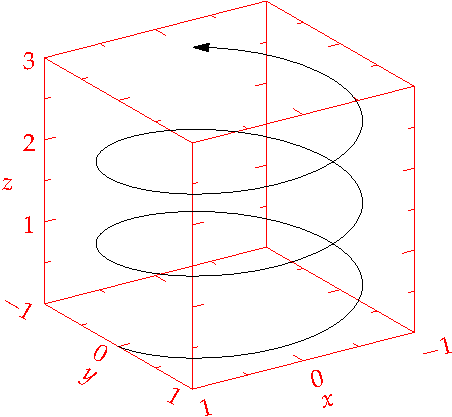
\includegraphics[width=\linewidth]{images/helix.pdf}
    \caption{margin figure}
    \label{app:fig:margin_fig}
    \end{marginfigure}

    \lipsum[1]

    \subsection{Figures} % (fold)
    \label{sub:figures}

    % subsection figures (end)

    \begin{figure}
        \centering
        \begin{subfigure}[b]{0.3\textwidth}
            \centering
            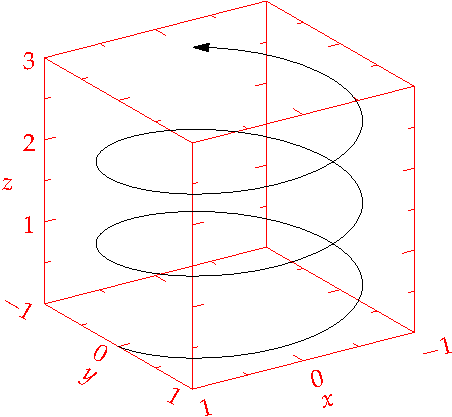
\includegraphics[width=\textwidth]{images/helix.pdf}
            \caption{subcaption 1}
            \label{fig:1}
        \end{subfigure}
        \hfill
        \begin{subfigure}[b]{0.3\textwidth}
            \centering
            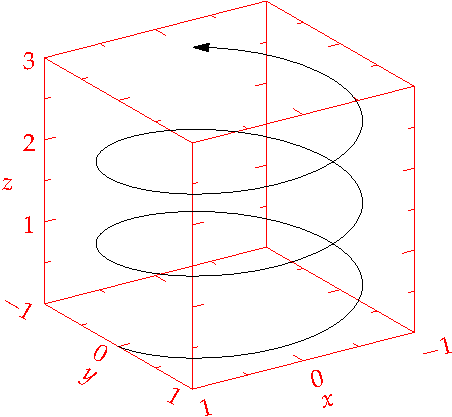
\includegraphics[width=\textwidth]{images/helix.pdf}
            \caption{subcaption 2}
            \label{fig:2}
        \end{subfigure}
        \hfill
        \begin{subfigure}[b]{0.3\textwidth}
            \centering
            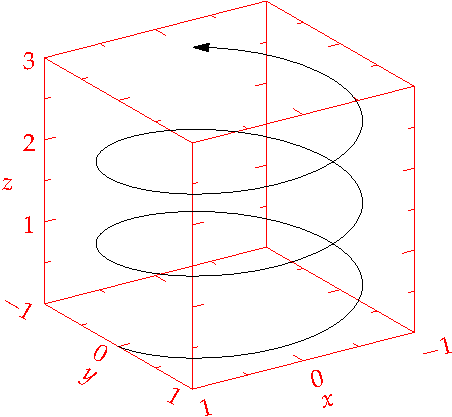
\includegraphics[width=\textwidth]{images/helix.pdf}
            \caption{subcaption 3}
            \label{fig:3}
        \end{subfigure}
        \caption{Example of figure with 3 subfigures}
        \label{fig:three_figs}
        % \setfloatalignment{b}  %b/t
        % \forceversofloat  % \forcerectofloat
    \end{figure}

    \begin{figure*}[h]
        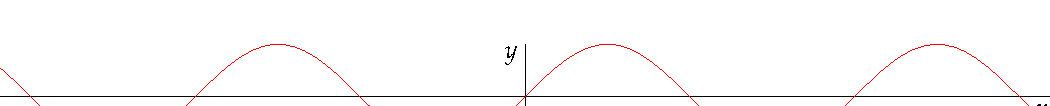
\includegraphics[width=\linewidth]{images/sine.pdf}%
        \caption{full width figure}%
        \label{app:fig:full_fig}%
    \end{figure*}

    \subsection{Equations} % (fold)
    \label{sub:equations}

        Normal equation
        \begin{equation}
        \label{eq:normal}
            \sum_{n=1}^{N} 1 / n \approx \ln(N).
        \end{equation}
        Full width equation
        \begin{fullwidth}
            \begin{equation}
            \label{eq:full_width}
                \sum_{n=1}^{N} 1 / n \approx \ln(N).
            \end{equation}
        \end{fullwidth}

        \newthought{There is also a custom command} \textsf{mathnote} to annotate equations.
        Its behavior is similar to \textsf{marginnote} but works in maths environments, like \textsf{equation} and \textsf{align}.
        I find it useful to make the transition between two steps of some derivations.
        Note that the equation number vanishes and the text is written in the margin.
        \begin{align}
            (x+1)^2
                &= (x+1)(x+1)
                \\
                &= x^2 + x + x + 1
                \quad\textsf{mathnote\{text\}\textbackslash\textbackslash}
                \mathnote{By developing the product}
                \\
                &= x^2 + 2x +1.
        \end{align}

        If you wish to preserve the equation number, you can combine the regular math environment with a manual teak of \textsf{marginnote} on a case-by-case basis.
        \marginnote{\text{ }\\[0.3em]Annotation}
        \begin{equation}
            \label{eq:annotated}
            \pi \approx 3.14
        \end{equation}

    % subsection equations (end)

    \subsection{Nomenclature, Glossary, Accronyms} % (fold)
    \label{sub:nomenclature_glossary_accronyms}

        \newthought{Indices}
            Fruits\index{fruits}, e.g.,
            orange\index{fruits!orange},
            banana\index{fruits!banana}
            apple\index{fruits!apple},
            kiwi\index{fruits!kiwi}

        \newthought{Acronyms}
            acrshort: \acrshort{gcd}, \acrshort{dpp}
            acrlong: \acrlong{gcd}, \acrlong{dpp}

        \newthought{Glossary}
            \Gls{tomato} \gls{tomato}
            \Glspl{tomato} \glspl{tomato}\\
            \Gls{dpp} \gls{dpp}

    % subsection nomenclature_glossary_accronyms (end)

% section examples (end)

\clearpage

\newthought{Below is a list of our contributions.}

\begin{fullwidth}
\textit{Journal paper(s)} % (fold)
% \label{par:journals}
    \begin{quote}
      \begin{itemize}
        \item[\paperIcon] \fullcite{Tufte2006}.
      \end{itemize}
    \end{quote}
\end{fullwidth}
% paragraph journals (end)

\begin{fullwidth}
\textit{Submitted to a journal} % (fold)
\label{par:working paper}
    \begin{quote}
      \begin{itemize}
        \item[\paperIcon] \fullcite{Tufte2006}.
      \end{itemize}
    \end{quote}
\end{fullwidth}
% textit working paper (end)

\begin{fullwidth}
\textit{Conference papers} % (fold)
\label{par:conferences}
    \begin{quote}
      \begin{itemize}
        \setlength{\itemsep}{5pt}
        \item[\conferenceIcon] \fullcite{Tufte2006}.
        \item[\conferenceIcon] \fullcite{Tufte2006}.
      \end{itemize}
    \end{quote}
\end{fullwidth}
% textit conferences (end)

\begin{fullwidth}
\textit{Workshop papers} % (fold)
\label{par:workshops}
    \begin{quote}
      \begin{itemize}
        \setlength{\itemsep}{5pt}
        \item[\conferenceIcon] \fullcite{Tufte2006}.
        \item[\conferenceIcon] \fullcite{Tufte2006}.
      \end{itemize}
    \end{quote}
\end{fullwidth}
% textit workshops (end)

\section{Outline of the manuscript} % (fold)
\label{sec:outline}

    \newthought{The manuscript is divided into five chapters.}

    \newthought{Chapter~\ref{ch:chapter_1}}
        lays the ground material for the subsequent chapters.

    \newthought{Chapter~\ref{ch:chapter_2}}
        discusses several methods available to

    \newthought{Chapter~\ref{ch:chapter_3}}
        discusses various methods to

    \newthought{Chapter~\ref{ch:chapter_4}}
        includes material accepted to

    \newthought{Chapter~\ref{ch:chapter_5}}
        includes material submitted to

    \newthought{The final section}
        contains a discussion

% section outline (end)

% chapter introduction (end)
  % Chapter 0

%!TEX root = ../main.tex

\chapter{Chapter}
\label{ch:chapter_1}

    \dochaptoc

% chapter chapter_1 (end)


% !TEX root = ../main.tex

\chapter{Chapter}
\label{ch:chapter_2}

    \dochaptoc

% chapter chapter_2 (end)


%!TEX root = ../main.tex

\chapter{Chapter}
\label{ch:chapter_3}

    \dochaptoc

% chapter chapter_3 (end)


%!TEX root = ../main.tex

\chapter{Chapter}
\label{ch:chapter_4}

    \dochaptoc

% chapter chapter_4 (end)


%!TEX root = ../main.tex

\chapter{Chapter}
\label{ch:chapter_5}

\dochaptoc

% chapter chapter_5 (end)


%%%%%%%%%%%%%%%%%%%%%%%%%%%%%%%%%%%%%%%%%%%%%%%%%%%%%%%%%%%%%%%%%%%%%%%%%%
% The back matter contains unnumbered chapters
% conclusion, french summary, bibliographies, indices, glossaries
%%%%%%%%%%%%%%%%%%%%%%%%%%%%%%%%%%%%%%%%%%%%%%%%%%%%%%%%%%%%%%%%%%%%%%%%%%

\backmatter

%!TEX root = ../main.tex

\chapter{Discussion} % (fold)
\label{ch:conclusion}

% chapter conclusion (end)

%!TEX root = ../main.tex

\chapter*{Résumé en français} % (fold)
\label{ch:french_resume}

\addcontentsline{toc}{chapter}{Résumé en français}

% chapter french_resume (end)

\begin{fullwidth}
    \printbibliography[heading=bibintoc]
\end{fullwidth}

\begin{fullwidth}
    \printindex
\end{fullwidth}

\begin{fullwidth}
    \printglossary[type=\acronymtype]
    \printglossary
\end{fullwidth}

%!TEX root = ../main.tex

\clearpage

\paragraph{English abstract} % (fold)
\label{par:english_abstract}

\textbf{Keywords:}

% paragraph english_abstract (end)

\paragraph{French abstract} % (fold)
\label{par:french_abstract}

\textbf{Mots clés :}

% paragraph french_abstract (end)


\end{document}
